% *********************************************************************
% © 2021–2024 Jeremy Sylvestre
%
% Permission is granted to copy, distribute and/or modify this document
% under the terms of the GNU Free Documentation License, Version 1.3 or
% any later version published by the Free Software Foundation; with no
% Invariant Sections, no Front-Cover Texts, and no Back-Cover Texts. A
% copy of the license is included in the appendix entitled “GNU Free
% Documentation License” that appears in the output document of this
% PreTeXt source code. All trademarks™ are the registered® marks of
% their respective owners.
%
% *********************************************************************

\newcommand*{\xmin}{-0.5}
\newcommand*{\xmax}{2}
\newcommand*{\ymin}{-0.5}
\newcommand*{\ymax}{8}

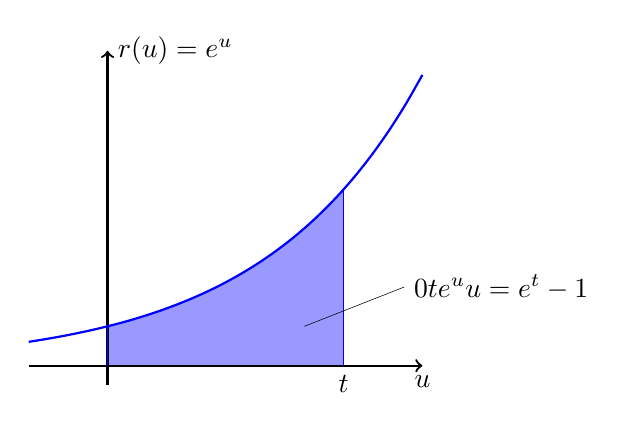
\begin{tikzpicture}
[
	closedpt/.style={circle,draw,fill,inner sep=0pt,minimum size=4pt},
	openpt/.style={circle,draw,inner sep=0pt,minimum size=4pt},
	yscale=0.5,xscale=2
]

	% fills
	\fill[blue!40!white] (1,1) plot[domain=0:1.5] (\x,{exp \x}) -- (1.5,0) -- (0,0) -- cycle;

	% axes
	\draw[->,thick] (\xmin,0) -- (\xmax,0) node[below] {$u$};
	\draw[->,thick] (0,\ymin) -- (0,\ymax) node[right] {$r(u) = e^u$};

	% graph
	\draw[thick, blue, domain=-0.5:2, smooth] plot (\x,{exp \x});
	\draw[blue] (0,1) -- (0,0);
	\draw[blue] (1.5,4.482) -- (1.5,0);
	\node[below] at (1.5,0) {$t$};

	\node at (2.5,2) (int) {$\displaystyle \ccmint{0}{t}{e^u}{u} = e^t - 1$};
	\draw[very thin] (int.west) -- (1.25,1);

\end{tikzpicture}
